\begin{center}
    \textbf{\Huge "OSN Korea" 2023 Nomor 1}\\
    \textbf{\large KMO Final Round 2023 Problem 1}
\end{center}

\newpage

\section{Soal}
\subsection{Soal Asli dalam Bahasa Korea}
\begin{center}
    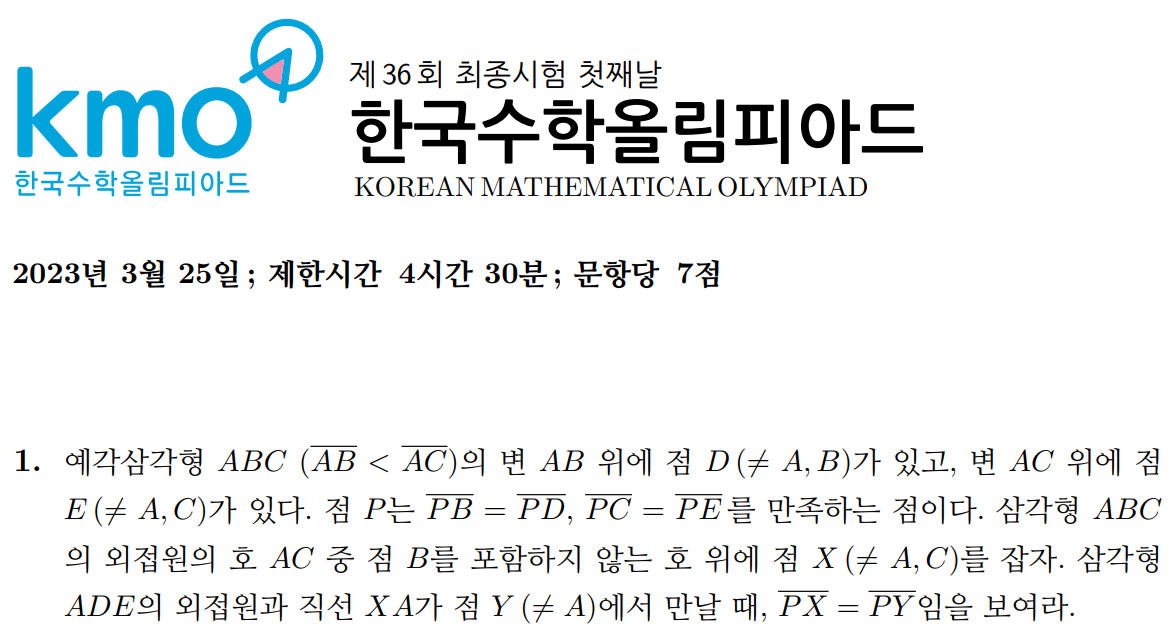
\includegraphics[scale=0.5]{0Figure/22-kmo2023p1}
\end{center}
\subsection{Soal Terjemahan}
Pada sebuah segitiga $ABC ~(AB<AC)$, titik $D (\neq A, B)$ dan $E (\neq A, C)$ terletak pada sisi $AB$ dan $AC$ berturut-turut. Titik $P$ memenuhi $PB=PD$ dan $PC=PE$. Titik $X (\neq A, C)$ terletak pada busur $AC$ pada lingkaran luar segitiga $ABC$ yang tidak memuat $B$. Misalkan $Y (\neq A)$ adalah perpotongan lingkaran luar $ADE$ dan garis $XA$. Buktikan bahwa $PX=PY$.

\newpage
\section{Solusi}
    Misalkan garis $DE$ memotong garis $BC$ di $F$. Perhatikan bahwa $BCED$ merupakan \textit{complete quadrilateral} sehingga berdasarkan teorema Miquel, lingkaran $(ADE)$, $(BDF)$, $(CEF)$, dan $(ABC)$ bertemu di satu titik, misalkan di titik $G$. 

    \begin{center}
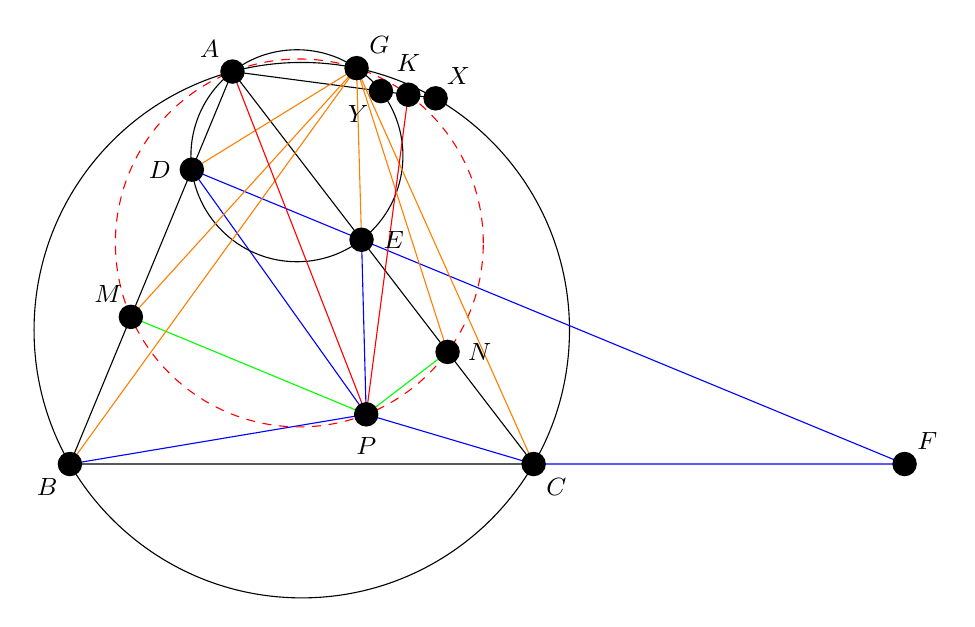
\begin{tikzpicture}[scale=3.4,line cap=round,line join=round]
  \draw[] (-0.25882,0.96593)--(-0.86603,-0.5)--(0.86603,-0.5)--(-0.25882,0.96593);
  \draw[blue] (-0.41062,0.59944)--(0.2407,-0.31438)--(-0.86603,-0.5);
  \draw[blue] (0.86603,-0.5)--(0.2407,-0.31438)--(0.22326,0.33767);
  \draw[green] (-0.63832,0.04972)--(0.2407,-0.31438)--(0.54464,-0.08116);
  \draw[] (0,0) circle (1);
  \draw[] (-0.01811,0.65154) circle (0.39595);
  \draw[dashed,red] (-0.00906,0.32577) circle (0.68715);
  \draw[] (-0.25882,0.96593)--(0.5,0.86603);
  \draw[blue] (-0.41062,0.59944)--(0.22326,0.33767)--(2.25167,-0.5)--(0.86603,-0.5);
  \draw[orange] (-0.41062,0.59944)--(0.20475,0.97881)--(0.22326,0.33767);
  \draw[orange] (-0.63832,0.04972)--(0.20475,0.97881)--(0.54464,-0.08116);
  \draw[orange] (-0.86603,-0.5)--(0.20475,0.97881)--(0.86603,-0.5);
  \draw[red] (-0.25882,0.96593)--(0.2407,-0.31438)--(0.39788,0.87947);
  \fill (-0.25882,0.96593) circle (1.3pt);
  \fill (-0.86603,-0.5) circle (1.3pt);
  \fill (0.86603,-0.5) circle (1.3pt);
  \fill (-0.41062,0.59944) circle (1.3pt);
  \fill (0.22326,0.33767) circle (1.3pt);
  \fill (-0.63832,0.04972) circle (1.3pt);
  \fill (0.54464,-0.08116) circle (1.3pt);
  \fill (0.2407,-0.31438) circle (1.3pt);
  \fill (0.5,0.86603) circle (1.3pt);
  \fill (0.29576,0.89291) circle (1.3pt);
  \fill (0.20475,0.97881) circle (1.3pt);
  \fill (2.25167,-0.5) circle (1.3pt);
  \fill (0.39788,0.87947) circle (1.3pt);
  \node[font=\small] at (-0.34367,1.05078) {$A$};
  \node[font=\small] at (-0.95088,-0.58485) {$B$};
  \node[font=\small] at (0.95088,-0.58485) {$C$};
  \node[font=\small] at (-0.53062,0.59944) {$D$};
  \node[font=\small] at (0.34326,0.33767) {$E$};
  \node[font=\small] at (-0.72318,0.13457) {$M$};
  \node[font=\small] at (0.66464,-0.08116) {$N$};
  \node[font=\small] at (0.2407,-0.43438) {$P$};
  \node[font=\small] at (0.58485,0.95088) {$X$};
  \node[font=\small] at (0.2109,0.80806) {$Y$};
  \node[font=\small] at (0.2896,1.06367) {$G$};
  \node[font=\small] at (2.33652,-0.41515) {$F$};
  \node[font=\small] at (0.39788,0.99947) {$K$};
\end{tikzpicture}
\end{center}


    Perhatikan bahwa $\dangle BGD = \dangle BFD = \dangle CFE = \dangle CGE$ dan $\dangle DBG = \dangle ABG = \dangle ACG = \dangle ECG$ yang menyebabkan $\triangle GDB \sim \triangle GEC$. Oleh karena itu, jika dimisalkan $M$ dan $N$ berturut-turut adalah titik-titik tengah dari $BD$ dan $CE$, maka $\triangle GDM \sim \triangle GEN$. Dari sini didapat $\dangle GMA = \dangle GMD = \dangle GNE = \dangle GNA$ yang mengimplikasikan $G,M,N,A$ siklis. 

    Di lain sisi, kita punya $\dangle YXG = \dangle AXG = \dangle ACG = \dangle ECG$ dan $\dangle GYX = \dangle GYA = \dangle GEA = \dangle GEC$ yang mengimplikasikan $\triangle GYX \sim \triangle GEC$. Oleh karena itu, jika $K$ adalah titik tengah $YX$, maka $\triangle GYK \sim \triangle GEN$ yang menyebabkan $\dangle GKA = \dangle GKY = \dangle GNE = \dangle GNA$ yang dengan kata lain mengakibatkan $G,A,K,N$ konsiklis.

    Terakhir, karena $DP=PB$ dan $M$ titik tengah $BD$, maka $PM \perp AM$. Dengan cara serupa didapat pula $PN \perp AN$. Dari sini mudah disimpulkan bahwa $AMPN$ siklis dengan $AP$ sebagai diameternya.
    
    Fakta-fakta tersebut mengantarkan kita pada fakta $A,K,N,P,M,G$ konsiklis dengan $AP$ sebagai diameter. Hal ini langsung membuat $PK \perp YX$. Karena $K$ adalah titik tengah $YX$ maka dapat disimpulkan bahwa $PY=PX$. Terbukti. 
